\documentclass[../thesis.tex]{subfiles}
 
\begin{document}
\vspace{-1\baselineskip}

Activity within the \acs{ATLAS} detector are recorded as raw electronic signals, which can be utilized by \acs{ATLAS} reconstruction software to derive physics objects for analysis. This chapter describes the reconstruction and identification of basic objects (e.g. interaction vertices, tracks, topological clusters of energy deposits) and subsequently of complex physics objects i.e. particles and particle signatures.

\section{Primary reconstruction}
\label{sec:primaryreco}

\subsection{Tracks}

Charged particles traveling through the ATLAS detector deposit energy in different layers of the \acs{ID} and \acs{MS}. The \acs{ID} track reconstruction software consists of two algorithm chains: inside-out and outside-in track reconstruction \citep{reco:track,reco:io,reco:oi}.

The inside-out algorithm is primarily used for the reconstruction of primary particles i.e. particles directly produced from $pp$ collisions or decay products of short-lived particles. The process starts by forming space points from seeded hits in the silicon detectors within the pixel \& \acs{SCT} detectors. Hits further away from the interaction vertex are added to the track candidate using a combinatorial Kalman filter \citep{reco:kalman} pattern recognition algorithm. Track candidates are then fitted with a \acs{chi2} filter \citep{reco:track_chi2} and loosely matched to a fixed-sized \acs{EM} cluster. Successfully matched track candidates are re-fitted with a Gaussian-sum filter (\acs{GSF}) \citep{reco:track_gsf}, followed by a track scoring strategy to resolve fake tracks \& hit ambiguity between different tracks \citep{reco:track_ambiguity}. The track candidate is then extended to the \acs{TRT} to form final tracks satisfying $\pT > 400$ MeV. The outside-in algorithm handles secondary tracks mainly produced from long-lives particles or decays of primary particles by back-tracking from \acs{TRT} segments, which are then extended inward to match silicon hits in the pixel and \acs{SCT} detectors to form track reconstruction objects.
% ms track reconstruction? \citep{reco:muon_ID2}

\subsection{Vertices}
\label{sec:vertex}
Vertices represent the point of interaction or decay for particles within the ATLAS detector. Primary vertices (\acs{PV}s) are defined as the point of collision for hard-scattering $pp$ interactions, while secondary or displaced vertices result from particle decays occurring at a distance from its production point. 

Reconstruction of \acs{PV}s is crucial to accurately profile the kinematic information of an event and form a basis for subsequent reconstruction procedures. Primary vertex reconstruction occurs in two stages: vertex finding and vertex fitting \citep{reco:vertex_primary}. The vertex finding algorithm uses the spatial coordinates of reconstructed tracks to form the seed for a vertex candidate. An adaptive vertex fitting algorithm \citep{reco:vertex_fitting} then iteratively evaluates track-vertex compatibility to estimate a new best vertex position. Less compatible tracks are down-weighted in each subsequent iteration, and incompatible tracks are removed and can be used for another vertex seed; the process is repeated until no further \acs{PV} can be found. All reconstructed vertices without at least two matched tracks are considered invalid and discarded.

Secondary vertex reconstruction uses the Secondary Vertex Finder (SVF) algorithm \citep{reco:vertex_secondary} which is primarily designed to reconstruct $b$- and $c$-hadrons for flavor tagging purposes. The SVF aims to reconstruct one secondary vertex per jet and only considers tracks that are matched to a two-track vertex and contained within a \pT-dependent cone around the jet axis. The tracks are then used to reconstruct a secondary vertex candidate using an iterative process similar to the \acs{PV} vertex fitting procedure.

\subsubsection*{Pile-up}
At high luminosities, multiple interactions can be associated with one bunch crossing, resulting in many \acs{PV}s. The effect is called pile-up, and usually result from soft \acs{QCD} interactions. Pile-up can be categorized into two types: in-time pile-up, stemming from additional $pp$ collisions in the same bunch crossing that is not the hard-scatter process; out-of-time pile-up, resulting from leftover energy deposits in the calorimeters from other bunch crossings \citep{reco:pileup}.
% Pile-up jets are usually from soft interactions and can be distinguished with JVT algorithm using tracking information from the ID.

\subsection{Topological clusters}
\label{sec:topocluster}
%\citep{reco:topocluster_2}\\
%Used to reconstruct hadronic objects and particles decaying hadronically i.e. $\tau$ leptons\\

Topological clusters (topo-clusters) \citep{reco:topocluster} consist of clusters of spatially related calorimeter cell signals. Topo-clusters are primarily used to reconstruct hadron- and jet-related objects in an effort to extract signal while minimizing electronic effects and physical fluctuations, and also allow for recovery of energy lost through bremsstrahlung or photon conversions. Cells with signal-to-noise ratio $\varsigma_\mathrm{cell}^\mathrm{EM}$ passing a primary seed threshold are seeded into a dynamic topological cell clustering algorithm as part of a proto-cluster. Neighboring cells satisfying a cluster growth threshold are collected into the proto-cluster. If a cell is matched to two proto-clusters, the clusters are merged. Two or more local signal maxima in a cluster satisfying $E_\mathrm{cell}^\mathrm{EM}>500$ MeV suggest the presence of multiple particles in close proximity, and the cluster is split accordingly to maintain good resolution of the energy flow. The process continues iteratively until all cells with $\varsigma_\mathrm{cell}^\mathrm{EM}$ above a principal cell filter level have been matched to a cluster.

\begin{figure}[!htbp]
\centering
\subfloat[Cells passing primary seed threshold]{
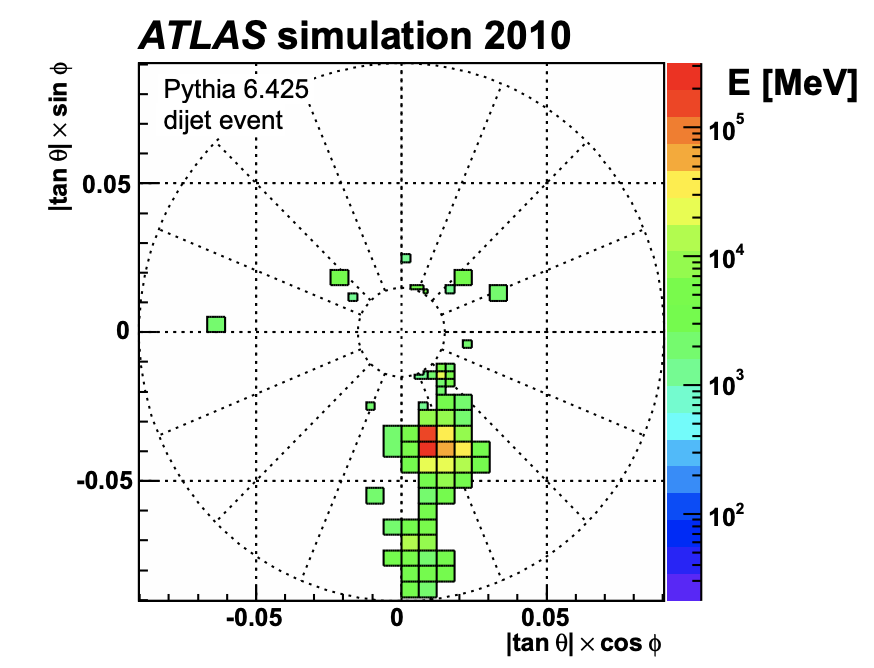
\includegraphics[width=0.5\linewidth]{fig/reco_topo1.png}}
\subfloat[Cells passing cluster growth threshold]{
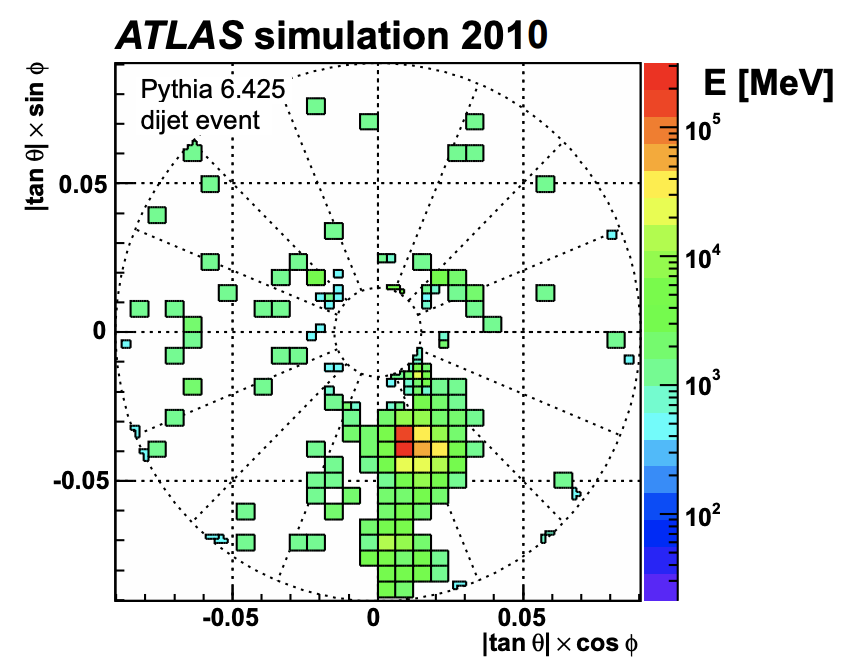
\includegraphics[width=0.5\linewidth]{fig/reco_topo2.png}}

\subfloat[Final reconstructed topo-clusters]{
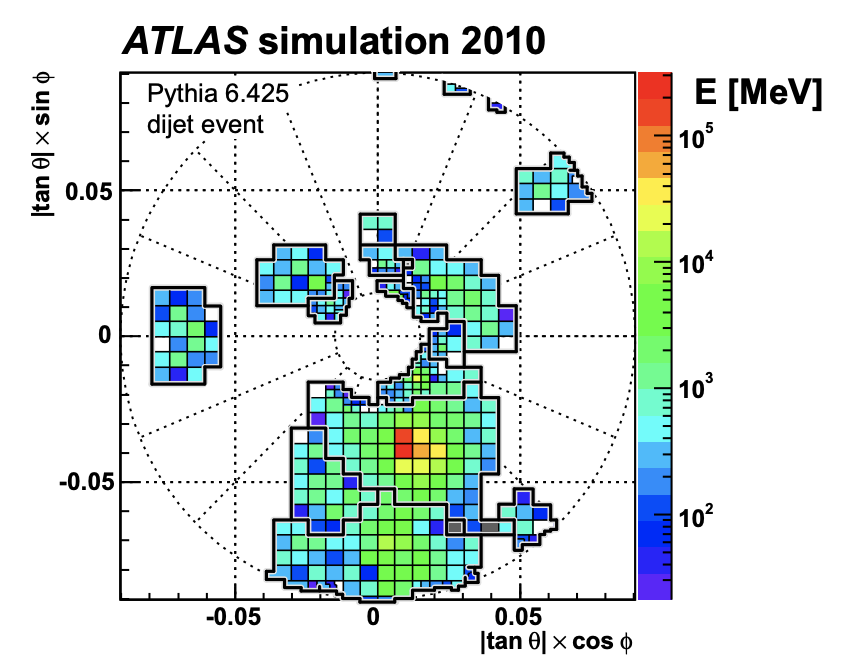
\includegraphics[width=0.5\linewidth]{fig/reco_topo3.png}}
\caption[Stages of topo-cluster formation corresponding to each threshold. In (a), proto-clusters are seeded from cells with adequate signal significance $\varsigma_\mathrm{cell}^\mathrm{EM}$. The clusters are further merged and split in (b) according to a predefined cluster growth threshold. The process stops in (c) when all sufficiently significant signal hits have been matched to a cluster.]{\label{fig:reco:topo1} Stages of topo-cluster formation corresponding to each threshold. In (a), proto-clusters are seeded from cells with adequate signal significance $\varsigma_\mathrm{cell}^\mathrm{EM}$. The clusters are further merged and split in (b) following a predefined cluster growth threshold. The process stops in (c) when all sufficiently significant signal hits have been matched to a cluster \citep{reco:topocluster}.}
\end{figure}

\section{Jets}
Quarks, gluons and other hadrons with non-neutral color charge cannot be observed individually due to \acs{QCD} color confinement, which forces a non-color-neutral hadron to almost immediately undergo hadronization, producing a collimated cone of color-neutral hadrons defined as a jet. Jet signals can be used to reconstruct and indirectly observe the quarks or gluons from which the jet originated in the original hard-scattering process.

\subsection{Jet reconstruction}

The ATLAS jet reconstruction pipeline is largely carried out using a particle flow (PFlow) algorithm combined with an anti-$k_t$ jet clustering algorithm. The PFlow algorithm \citep{reco:jet_pflow} utilizes topo-clusters along with information from both the calorimeter systems and the \acs{ID} in order to make use of the tracker system's advantages in low-energy momentum resolution and angular resolution. First, the energy from charged particles is removed from the calorimeter topo-clusters; then, it is replaced by particle objects created using the remaining energy in the calorimeter and tracks matched to topo-clusters. The ensemble of "particle flow objects" and corresponding matched tracks are used as inputs for the interative anti-$k_t$ algorithm \citep{reco:jet_antikt}.

The main components of the anti-$k_t$ algorithm involve the distance $d_{ij}$ between two jet candidates $i$ and $j$, and the distance $d_{iB}$ between the harder jet candidate of the two (defined as $i$) and the beamline $B$. If $d_{ij} < d_{iB}$, then the two jet candidates are combined and returned to the pool of candidates; otherwise, jet candidate $i$ is considered a jet and removed from the pool. The distance $d_{ij}$ is inversely proportional to a predefined radius parameter $\Delta R$ in order to control reconstruction quality for small-$R$ and large-$R$ jets. This analysis uses $\Delta R=0.4$ to better handle heavily collimated small-$R$ jets resulting from parton showers.

The anti-$k_t$ jets so far have only been reconstructed at the \acs{EM} level and need to be calibrated to match the energy scale of jets reconstructed at particle level. This is done via a \acs{MC}-based jet energy scale (\acs{JES}) calibration sequence, along with further calibrations to account for pile-up effects and energy leakage. The full \acs{JES} calibration sequence is shown in \autoref{fig:reco:jet_jes_calib}. All calibration except origin correction are applied to the jet's four-momentum i.e. jet \pT, energy and mass. Afterwards, a jet energy resolution (\acs{JER}) \citep{reco:jet_jer} calibration step is carried out in a similar manner to \acs{JES} to match the resolution of jets in dijet events.
To further suppress pile-up effects, a neural-network based jet vertex tagger (\acs{NNJvt}) discriminant was developed based on the previous jet vertex tagger (\acs{JVT}) algorithm \citep{reco:pileup} and applied to low-\pT reconstructed jets.

\begin{figure}[!htbp]
\begin{center}
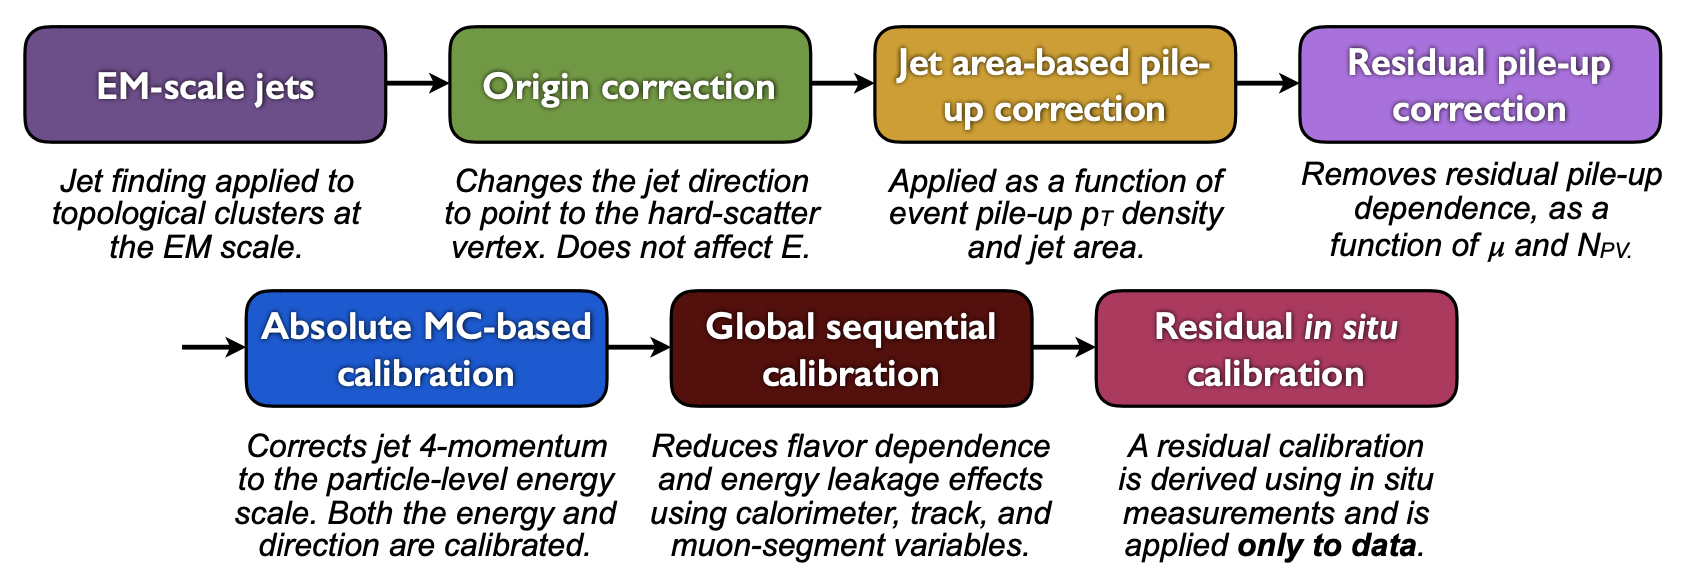
\includegraphics[width=\linewidth]{fig/reco_jet_jes_calib.png}
\caption[Jet energy scale calibration sequence for EM-scale jets.]{\label{fig:reco:jet_jes_calib}Jet energy scale calibration sequence for \acs{EM}-scale jets \citep{reco:jet_jes}.}
\end{center}
\end{figure}


\subsection{Flavor tagging}
\label{sec:ftag}
Identifying and classifying hadronic jets are important tasks for ATLAS physics, for example analyses involving Higgs decays $H\rightarrow b\bar{b}$ or top quarks. Flavor tagging or $b$-tagging is the process of identifying jets containing $b$-hadrons, $c$-hadrons, light-hadrons ($uds$-hadrons) or jets from hadronically decaying $\tau$ leptons. Distinguishing $b$-jets is of particular interest due to their characteristically long lifetime ($\tau\approx 1.5$ ps), displaced secondary decay vertex and high decay multiplicity.

Usage of $b$-tagging in this analysis is done via five operating points (\acs{OP}s), corresponding to 65\%, 70\%, 77\%, 85\% and 90\% $b$-jet tagging efficiency $\varepsilon_b$ in simulated \ttbar events, in order from the loosest to tightest discriminant cut point.
The \acs{OP}s are defined by placing selections on the tagger output to provide a predefined $\varepsilon_b$ level; the selection cuts act as a variable trade-off between $b$-tagging efficiency and $b$-jet purity i.e. $c$- or light-jet rejection. For this thesis, a jet is considered $b$-tagged if it passes the $85\%$ \acs{OP}. The $b$-tagged jet is then assigned a pseudo-continuous $b$-tagging (\acs{PCBT}) score, which quantifies a jet's ability to satisfy different \acs{OP}s. The score can take integer values between 1 and 6, where a score of 6 is assigned to jets passing all \acs{OP} thresholds; a score of 2 for jets that pass only the tightest OP (90\%); and a score of 1 for jets that pass no \acs{OP}. A value of -1 is also defined for any jet that does not satisfy $b$-tagging criteria. 

\subsubsection*{GN2 $b$-tagging algorithm}
\label{sec:gn2}

\begin{figure}[!htbp]
\begin{center}
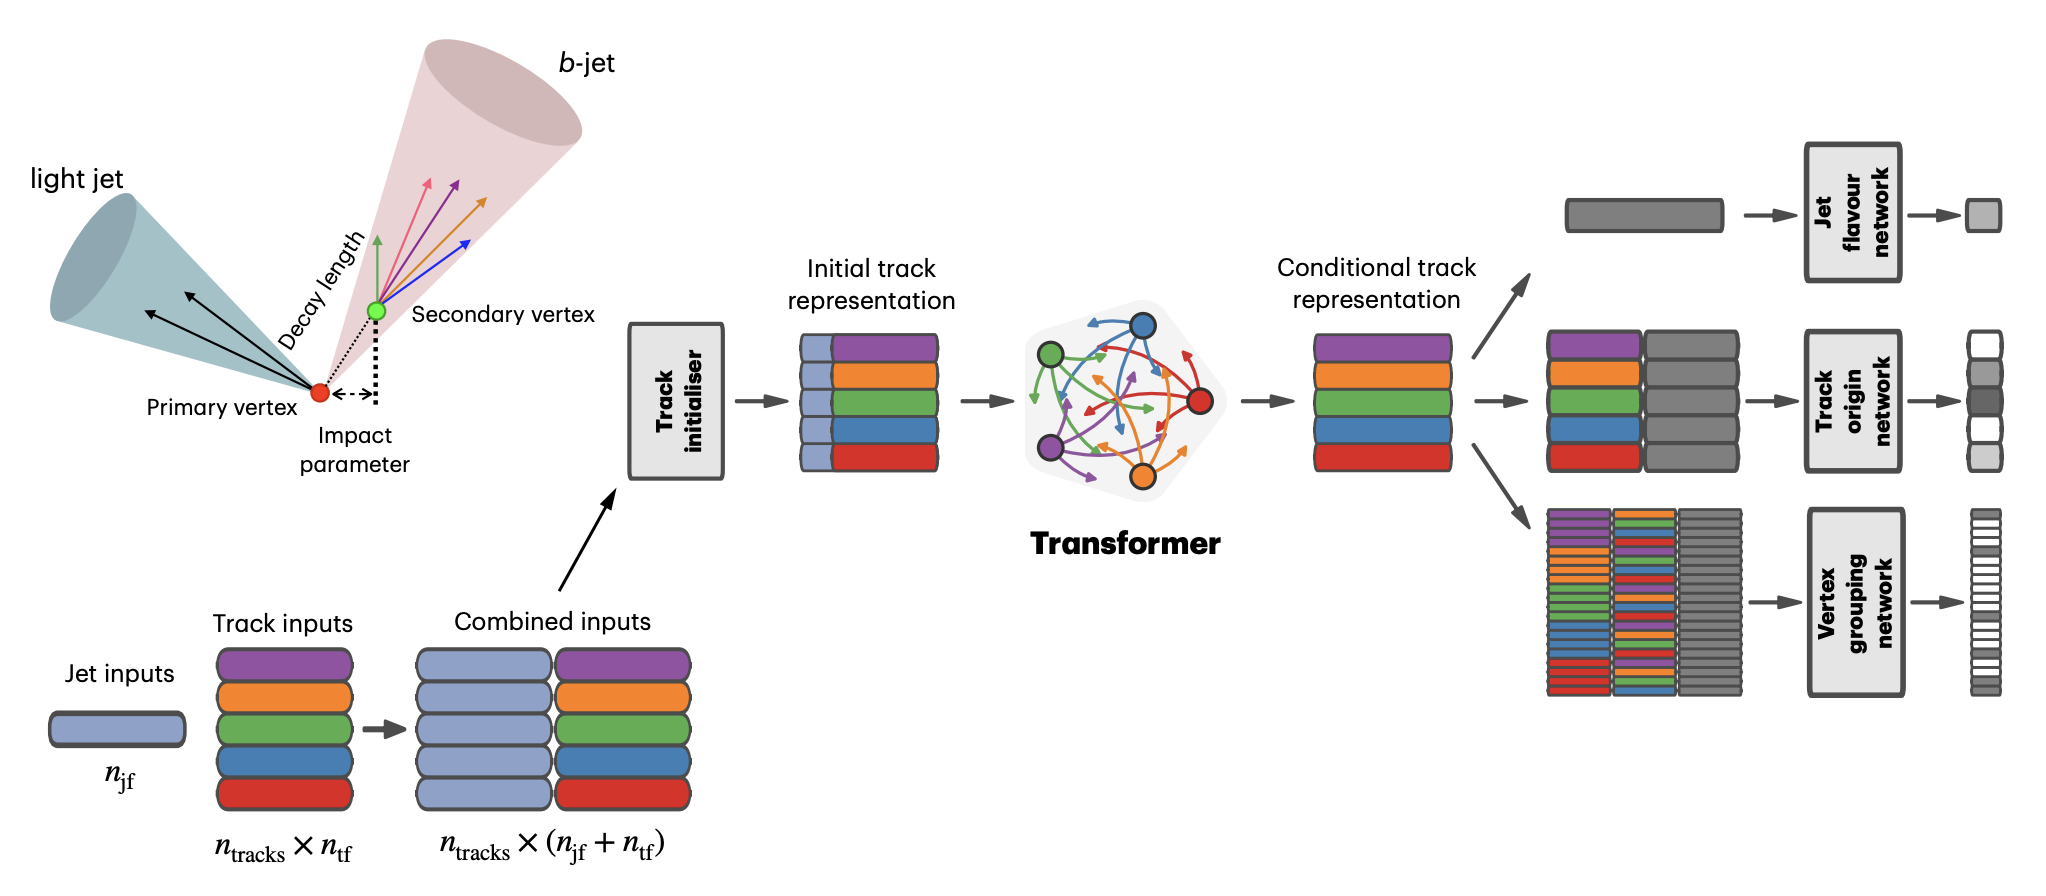
\includegraphics[width=\linewidth]{fig/reco_ftag_gn2.png}
\caption[Overview of the GN2 architecture. The number of jet and track features are represented by $n_\text{jf}$ and $n_\text{tf}$ respectively. The global jet representation and track embeddings output by the Transformer encoder are used as inputs for three task-specific networks.]{\label{fig:ftag:gn2}Overview of the GN2 architecture. The number of jet and track features are represented by $n_\text{jf}$ and $n_\text{tf}$ respectively. The global jet representation and track embeddings output by the Transformer encoder are used as inputs for three task-specific networks \citep{ftag:gn2}.}
\end{center}
\end{figure}
For this analysis, $b$-jets are identified and tagged with the GN2v01 $b$-tagger \citep{ftag:gn2}. The GN2 algorithm uses a Transformer-based model \citep{ftag:transformer} modified to incorporate domain knowledge and additional auxiliary physics objectives: grouping tracks with a common vertex and predicting the underlying physics process for a track. The network structure is shown in \autoref{fig:ftag:gn2}. The GN2 $b$-tagger form the input vector by concatenating 2 jet variables and 19 track reconstruction variables (for up to 40 tracks), normalized to zero mean and unit variance. The output consists of a track-pairing output layer of size 2, a track origin classification layer of 7 categories, and a jet classification layer of size 4 for the probability of each jet being a $b$-, $c$-, light- or $\tau$-jet respectively. For $b$-tagging purpose, a discriminant is defined using these four outputs
\begin{equation}
D_b = \ln \left( \displaystyle\frac{p_b}{f_c p_c + f_\tau p_\tau + (1-f_c-f_\tau) p_\text{light}} \right)
\end{equation}
where $p_x$ is the probability of the jet being an $x$-jet as predicted by GN2, and $f_c$, $f_\tau$ are tunable free parameters controlling balance between $c$- and light-jet rejection.

Simulated \acs{SM} \ttbar and \acs{BSM} $Z'$ events from $pp$ collisions were used as training and evaluation samples. In order to minimize bias, both $b$- and light-jet samples are re-sampled to match $c$-jet distributions. \autoref{fig:ftag:gn2_beff} shows the performance of GN2 compared to the previous convolutional neural network-based standard $b$-tagging algorithm DL1d, in terms of $c$-, light- and $\tau$-jet rejection as a function of $b$-tagging efficiency. The network gives a factor of 1.5-4 improvement in experimental applications compared to DL1d \citep{ftag:gn2}, without dependence on the choice of MC event generator or inputs from low-level flavor tagging algorithm.

\begin{figure}[!htb]
\centering
\subfloat[\ttbar sample]{
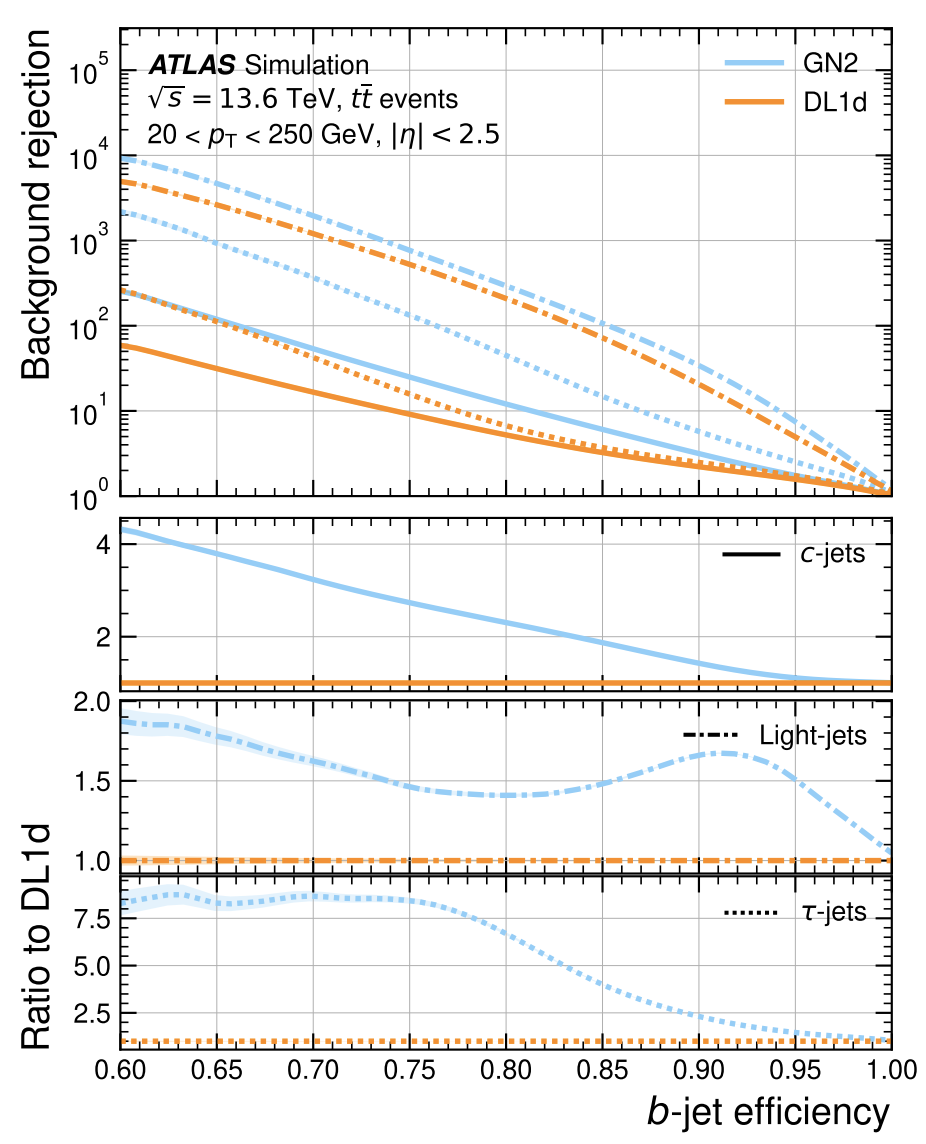
\includegraphics[width=0.5\linewidth]{fig/reco_ftag_gn2_ttbar.png}}
\subfloat[$Z'$ sample]{
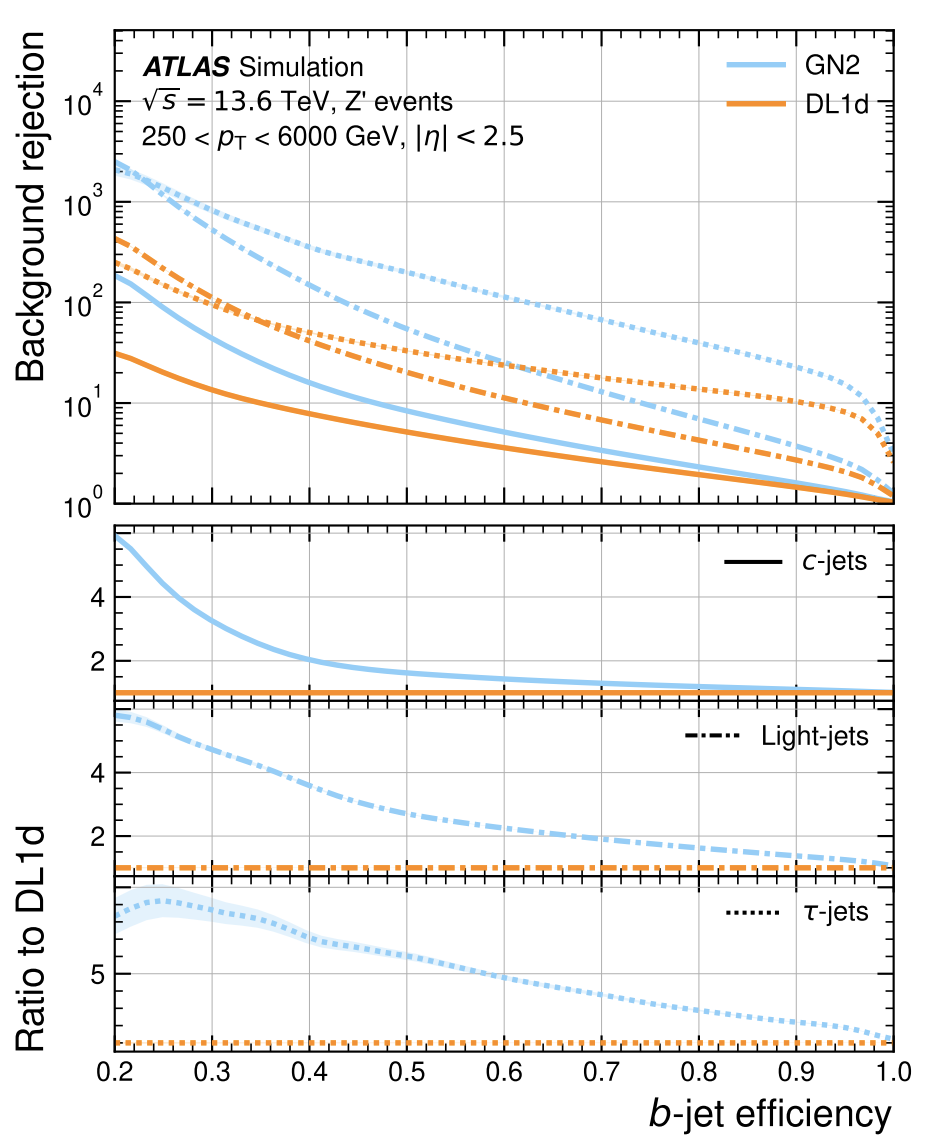
\includegraphics[width=0.5\linewidth]{fig/reco_ftag_gn2_zp.png}}
\caption[The $c$-, light- and $\tau$-jet rejection rate as a function of $b$-tagging efficiency for GN2 and DL1d using (a) jets in the \ttbar sample, and (b) jets in the $Z'$ sample. The performance ratios of GN2 to DL1d are shown in the bottom panels.]{\label{fig:ftag:gn2_beff}The $c$-, light- and $\tau$-jet rejection rate as a function of $b$-tagging efficiency for GN2 and DL1d using (a) jets in the \ttbar sample, and (b) jets in the $Z'$ sample. The performance ratios of GN2 to DL1d are shown in the bottom panels \citep{ftag:gn2}.}
\end{figure}

\subsubsection*{Efficiency calibration}
% \citep{ftag:gn1}\\
Due to imperfect description of detector response and physics modeling effects in simulation, the $b$-tagging efficiency predicted by \acs{MC} simulation $\varepsilon_b^\mathrm{sim}$ requires a correction factor to match the efficiency measured in collision data $\varepsilon_b^\mathrm{data}$. The correction scale factors (\acs{SF}s) are defined as $\mathrm{SF}=\varepsilon_b^\mathrm{data}/\varepsilon_b^\mathrm{sim}$ and are determined by data-to-\acs{MC} calibration using samples enriched in dileptonic \ttbar decays \citep{ftag:calib}. The resulting \acs{SF}s are applied to \acs{MC} simulated jets individually.


\section{Leptons}
Lepton reconstruction in ATLAS involves electron and muon reconstruction since tau decays quickly, and depending on decay mode can be reconstructed using either jets or light leptons.  Leptons can be classified into two categories: prompt leptons resulting from heavy particle decays and non-prompt leptons resulting from detector or reconstruction effects, or from heavy-flavor hadron decays.

\subsection{Electrons}
\label{sec:electron}
%- \citep{reco:electron_meas}\\
Electrons leave energy signature in the detector by interacting with the detector materials and losing energy in the form of bremsstrahlung photons. A bremsstrahlung photon can produce an electron-positron pair which can itself deposit signals in the detector, creating a cascade of particles that can leave multiple of either tracks in the \acs{ID} or \acs{EM} showers in the calorimeters, all of which are considered part of the same \acs{EM} topo-cluster. Electron signal signature has three characteristic components: localized energy deposits in the calorimeters, multiple tracks in the \acs{ID} and compatibility between the above tracks and energy clusters in the $\eta \times \phi$ plane \citep{reco:electron_id}. Electron reconstruction in ATLAS follows these steps accordingly.
%- Electron path through the detector is shown in \autoref{fig:reco:electron}

Seed-cluster reconstruction and track reconstruction are performed sequentially in accordance with the iterative topo-clustering algorithm and track reconstruction method described in \autoref{sec:primaryreco}. The seed-cluster and \acs{GSF}-refitted track candidate not associated with a conversion vertex are matched to form an electron candidate. The cluster energy is then calibrated using multivariate techniques on data and simulation to match the original electron energy.

\subsubsection*{Electron identification}
Additional \acs{LH}-based identification selections using \acs{ID} and \acs{EM} calorimeter information are implemented to further improve the purity of reconstructed electrons in the central region of the detector ($|\eta|<2.47$) \citep{reco:electron_id}. The electron \acs{LH} function is built with the signal being prompt electrons and background being objects with similar signature to prompt electrons i.e. hadronic jet deposits, photon conversions or heavy-flavor hadron decays. Three identification \acs{OP}s are defined for physics analyses: \textit{Loose}, \textit{Medium} and \textit{Tight}, optimized for 9 bins in $|\eta|$ and 12 bins in \ET with each \acs{OP} corresponding to a fixed efficiency requirement for each bin. For typical \acs{EW} processes, the target efficiencies for \textit{Loose}, \textit{Medium} and \textit{Tight} start at 93\%, 88\% and 80\% respectively and increase with \ET. Similar to $b$-tagging \acs{OP}s, the electron identification {OP}s represent a trade-off in signal efficiency and background rejection. The electron efficiency are estimated using tag-and-probe method on samples of $J/\Psi \rightarrow ee$ and $Z \rightarrow ee$ \citep{reco:electron_id}.
%The analysis in this thesis uses Tight electron identification requirement.
%\begin{figure}[!htbp]
%\centering
%\subfloat[Figure A]{
%\label{fig:a}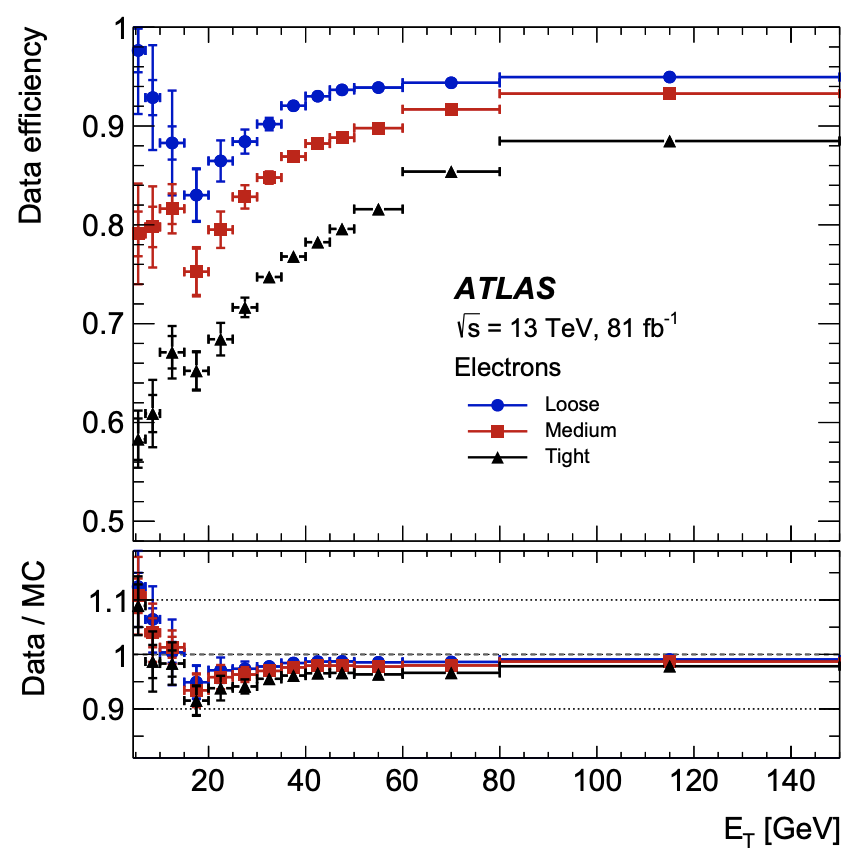
\includegraphics[width=0.5\linewidth]{fig/reco_electron_eff_ET.png}}
%\subfloat[Figure B]{
%\label{fig:b}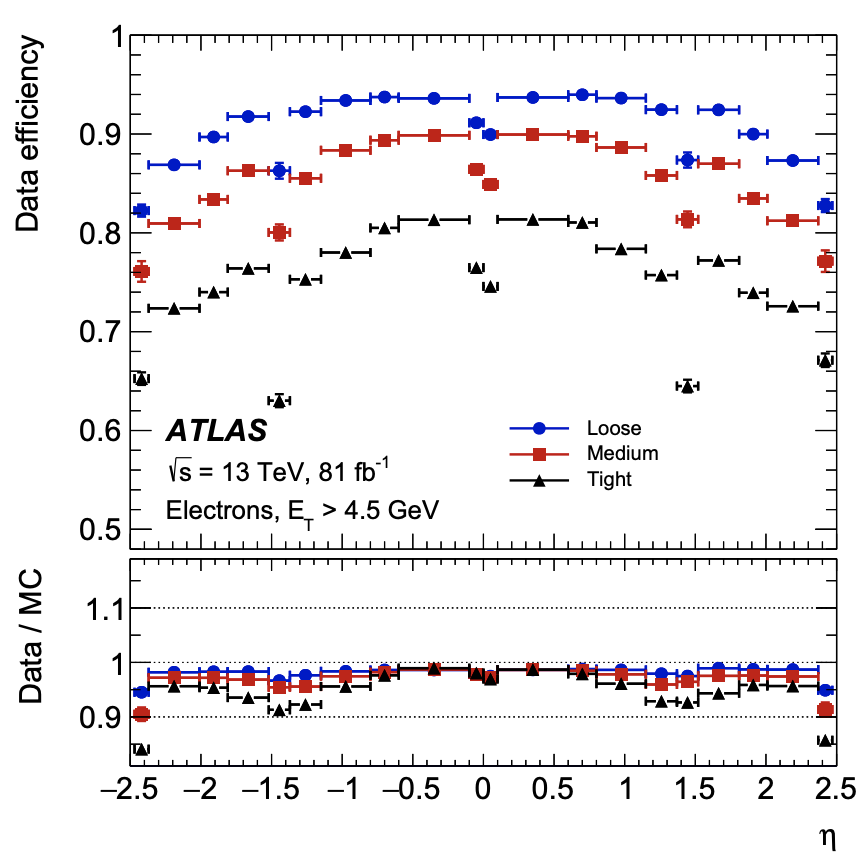
\includegraphics[width=0.5\linewidth]{fig/reco_electron_eff_eta.png}}
%\caption{\label{fig:reco:electron_eff}}
%\end{figure}

\subsubsection*{Electron isolation}
\label{sec:eiso}
A characteristic distinction between prompt electrons and electrons from background processes is the relative lack of activity in both the \acs{ID} and calorimeters within an $\Delta \eta \times \Delta \phi$ area surrounding the reconstruction candidate. Calorimeter-based and track-based electron isolation variables \citep{reco:electron_id} are defined to quantify the amount of activity around the electron candidate using topo-clusters and reconstructed tracks respectively.

Calorimeter-based isolation variables $E_\mathrm{T}^{\mathrm{cone}XX}$ are computed by first summing the energy of topo-clusters with barycenters falling within a cone of radius $\Delta R = \sqrt{(\Delta \eta)^2+(\Delta \phi)^2}=XX/100$ around the direction of the electron candidate. The final isolation variables are obtained by subtracting from the sum the energy belonging to the candidate electron at the core of the cone, then applying corrections for pile-up effects and energy leakage outside of the core. Similar to calorimeter-based variables, track-based isolation variables $p_\mathrm{T}^{\mathrm{varcone}XX}$ are calculated by summing all track \pT within a cone of radius $\Delta R$ around the electron candidate, minus the candidate's contribution. The cone radius is variable as a function of \pT and is described as

\begin{equation}
\Delta R \equiv \min \left(\frac{10}{\pT}, \Delta R_{\max} \right),
\end{equation}
where \pT is expressed in GeV and $\Delta R_{\max}$ is the maximum cone size, defined to account for closer proximity of decay products to the electron in high-momentum heavy particle decays. Four isolation operating points are implemented to satisfy specific needs by physics analyses: \textit{Loose}, \textit{Tight}, \textit{HighPtCaloOnly} and \textit{Gradient} \citep{reco:electron_id}.
%For this thesis, electrons isolation using Tight requirements.

%\begin{figure}[!htbp]
%\centering
%\subfloat[Figure A]{
%\label{fig:a}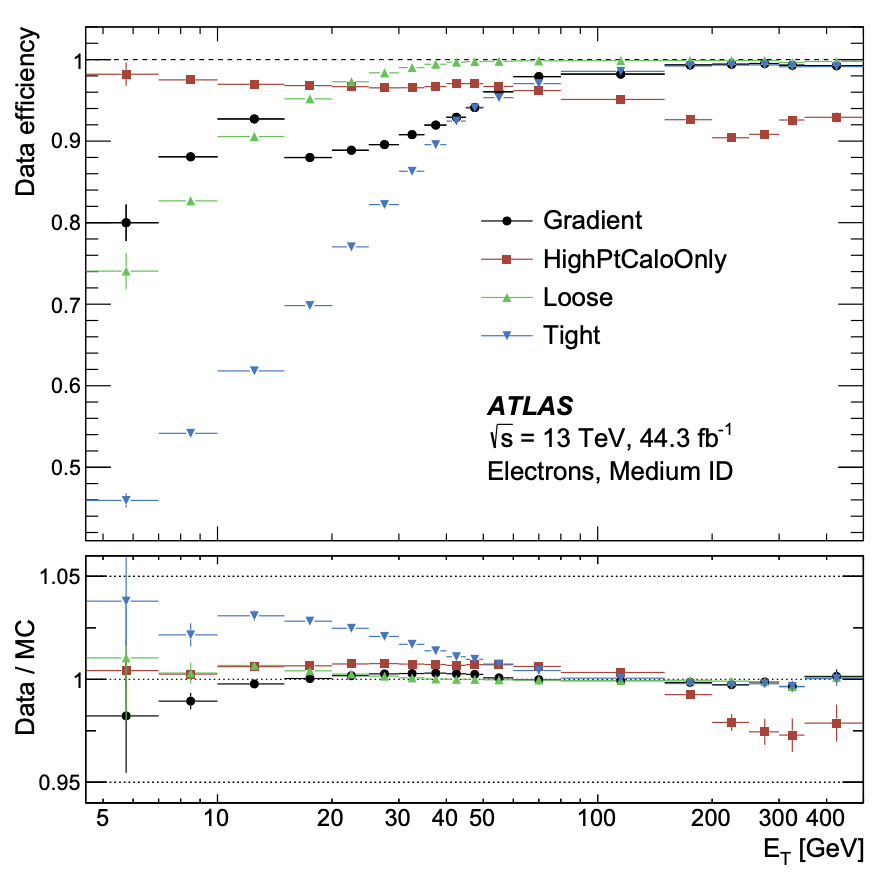
\includegraphics[width=0.5\linewidth]{fig/reco_electron_iso_ET.png}}
%\subfloat[Figure B]{
%\label{fig:b}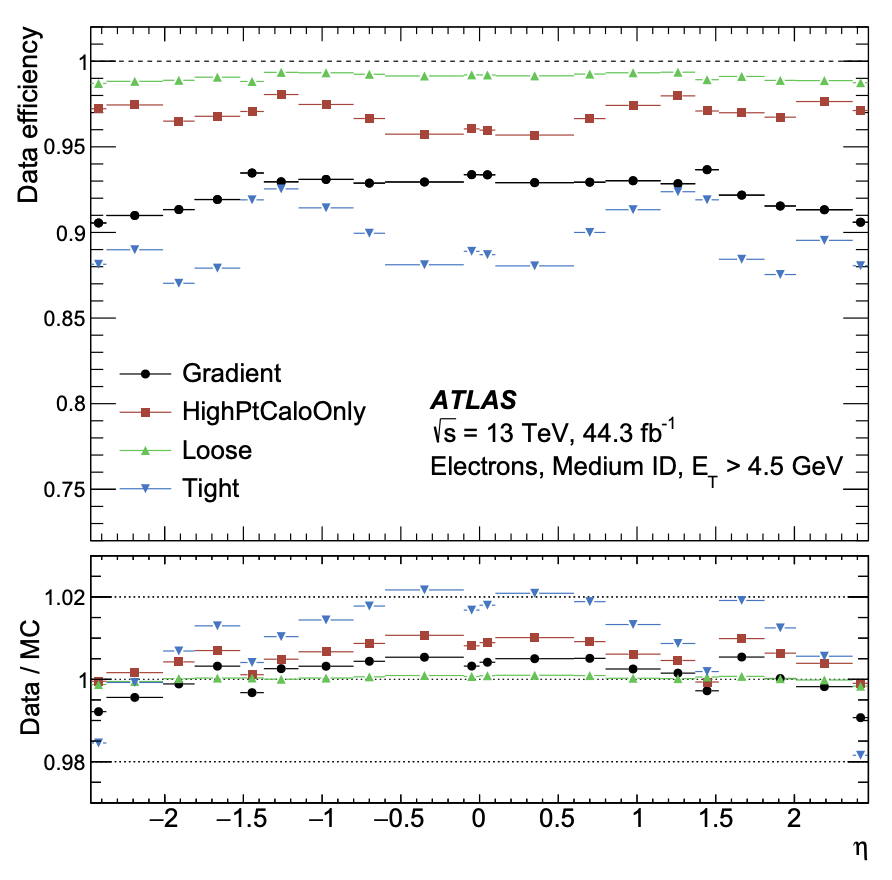
\includegraphics[width=0.5\linewidth]{fig/reco_electron_iso_eta.png}}
%\caption{\label{fig:reco:electron_iso}}
%\end{figure}

\subsubsection*{Electron charge misidentification}
Charge misidentification is a crucial irreducible background, particularly for analyses with electron charge selection criteria. Electron charge is determined by the curvature of the associated reconstructed track, and misidentification of charge can occur via either an incorrect curvature measurement or an incorrectly matched track. Inaccurate measurement is more likely for high energy electrons due to the small curvature in track trajectories at high \pT, while track matching error usually results from bremsstrahlung pair-production generating secondary tracks in close proximity \citep{reco:electron_id}. Suppression of this background is assisted via a boosted decision tree discriminant named the Electron Charge ID Selector (\acs{ECIDS}) \citep{reco:qmisid_cnn}. The addition of \acs{ECIDS} removed 90\% of electrons with incorrect charge while selecting 98\% of electrons with correct charge from electrons in $Z\rightarrow ee$ events satisfying \textit{Medium}/\textit{Tight} identification and \textit{Tight} isolation criteria.
%\begin{figure}[!htbp]
%\centering
%\subfloat[Figure A]{
%\label{fig:a}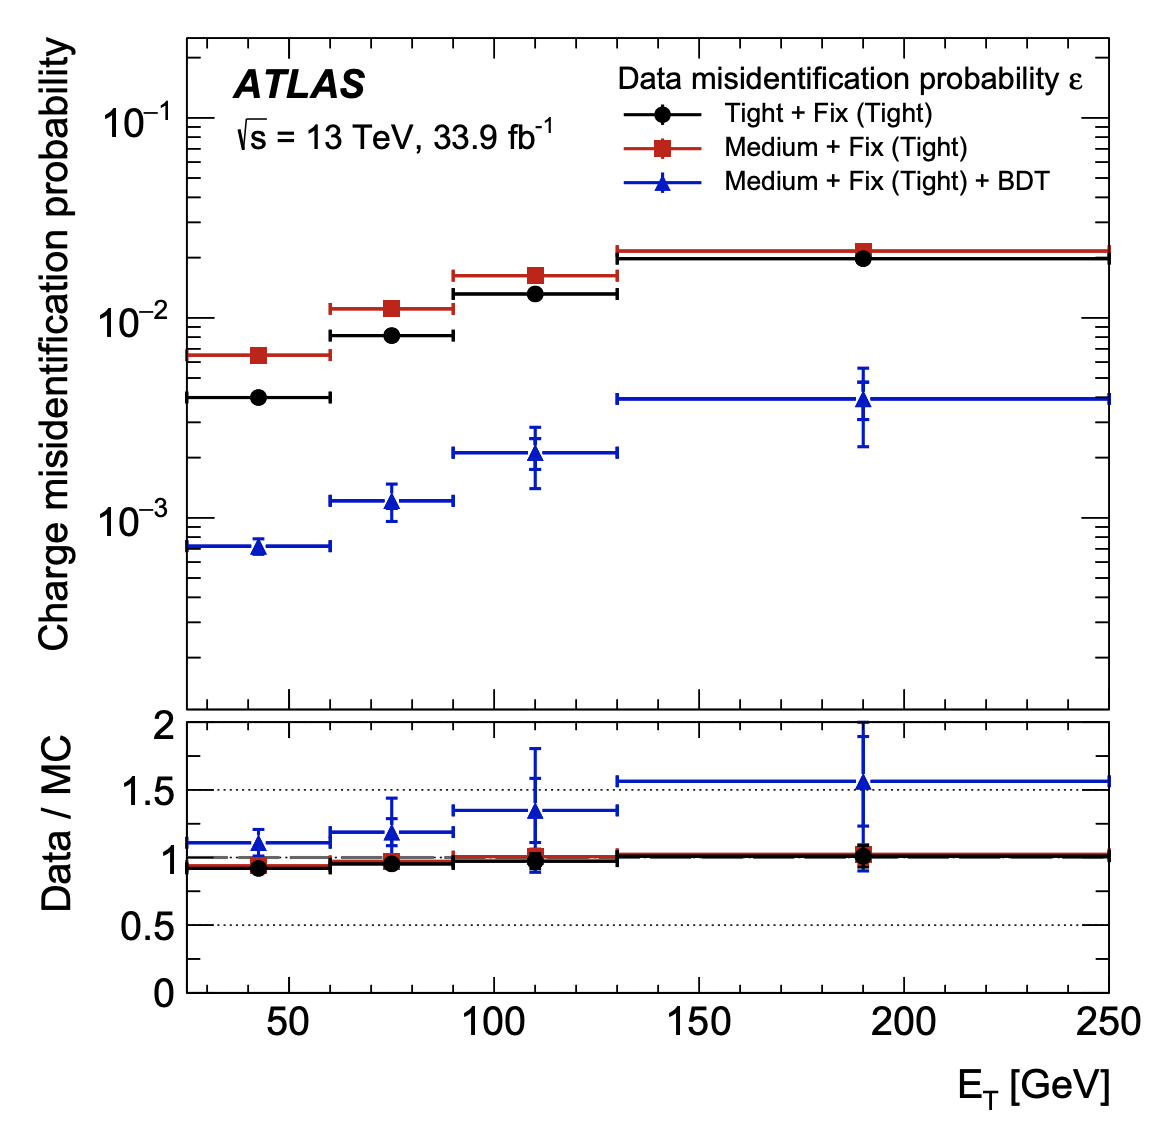
\includegraphics[width=0.5\linewidth]{fig/reco_qmisid_ET.png}}
%\subfloat[Figure B]{
%\label{fig:b}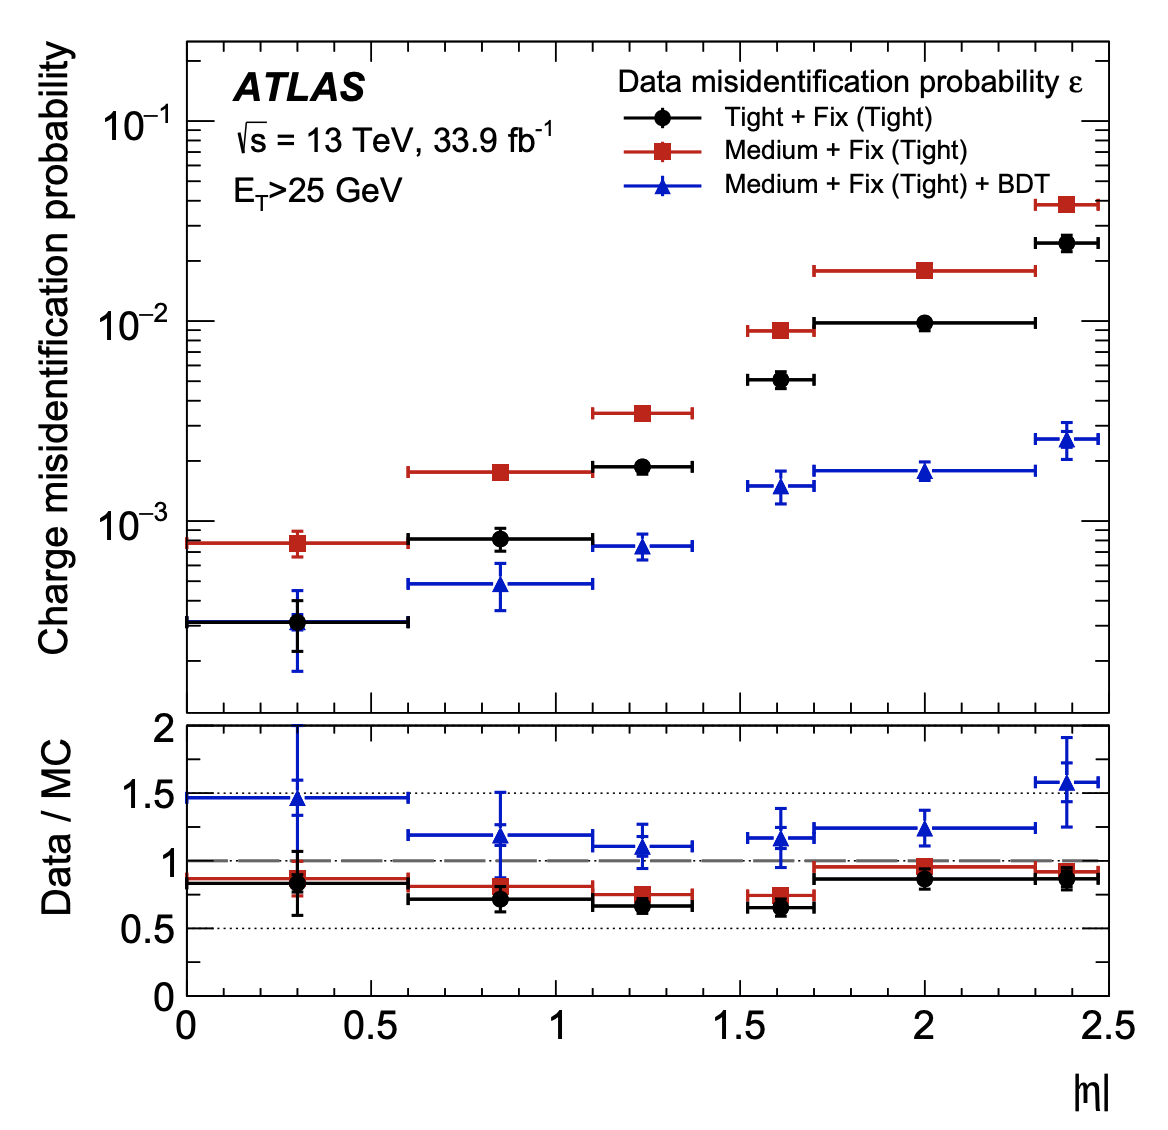
\includegraphics[width=0.5\linewidth]{fig/reco_qmisid_eta.png}}
%\caption[Caption]{\label{fig:reco:electron_iso}Caption \citep{reco:electron_meas}}
%\end{figure}


\subsection{Muons}
Muons act as minimum-ionizing particles, leaving tracks in the \acs{MS} or characteristics energy deposits in the calorimeter and can be reconstructed globally using information from the \acs{ID}, \acs{MS} and calorimeters. Five reconstruction strategies corresponding to five muon types \citep{reco:muon_ID} are utilized in ATLAS:
\begin{itemize}
\item Combined (CB): the primary ATLAS muon reconstruction method. Combined muons are first reconstructed using \acs{MS} tracks then extrapolated to include \acs{ID} tracks (outside-in strategy). A global combined track fit is performed on both \acs{MS} and \acs{ID} tracks.
\item Inside-out combined (IO): complementary to CB reconstruction. IO muon tracks are extrapolated from \acs{ID} to \acs{MS}, then fitted with \acs{MS} hits and calorimeter energy loss in a combined track fit.
\item \acs{MS} extrapolated (ME): ME muons are defined as muons with a \acs{MS} track that cannot be matched to an \acs{ID} track using CB reconstruction. ME muons allow extension of muon reconstruction acceptance to regions not covered by the ID ($2.5<|\eta|<2.7$)
\item Segment-tagged (ST): ST muons are defined as a successfully matched \acs{ID} track that satisfies tight angular matching criteria to at least one reconstructed \acs{MDT} or \acs{CSC} segment when extrapolated to the \acs{MS}. MS reconstruction is used primarily when muons only crossed one layer of MS chambers.
\item Calorimeter-tagged (CT): CT muons are defined as an \acs{ID} track that can be matched to energy deposits consistent with those of a minimum-ionizing particle when extrapolated through the calorimeter. CT reconstruction extends acceptance range to regions in the \acs{MS} with sparse instrumentation ($|\eta|<0.1$) with a higher \pT threshold of 5 GeV, compared to the 2 GeV threshold used by other muon reconstruction algorithms due to large background contamination at the low \pT range of $15 < \pT < 100$ GeV \citep{reco:muon_ID2}.
\end{itemize}
\subsubsection*{Muon identification}
%\citep{reco:muon_ID2}\\
Reconstructed muons are further filtered by identification criteria to select for high-quality prompt muons. Requirements include number of hits in the \acs{MS} and \acs{ID}, track fit properties and compatibility between measurements of the two systems. Three standard \acs{OP}s (\textit{Loose}, \textit{Medium}, \textit{Tight}) are defined to better match the needs of different physics analyses concerning prompt muon \pT resolution, identification efficiency and non-prompt muon rejection. The default identification \acs{OP} for ATLAS physics is \textit{Medium} which provides efficiency and purity suitable for a wide range of analyses while minimizing systematic uncertainties \citep{reco:muon_ID}.

%\begin{figure}[!htbp]
%\centering
%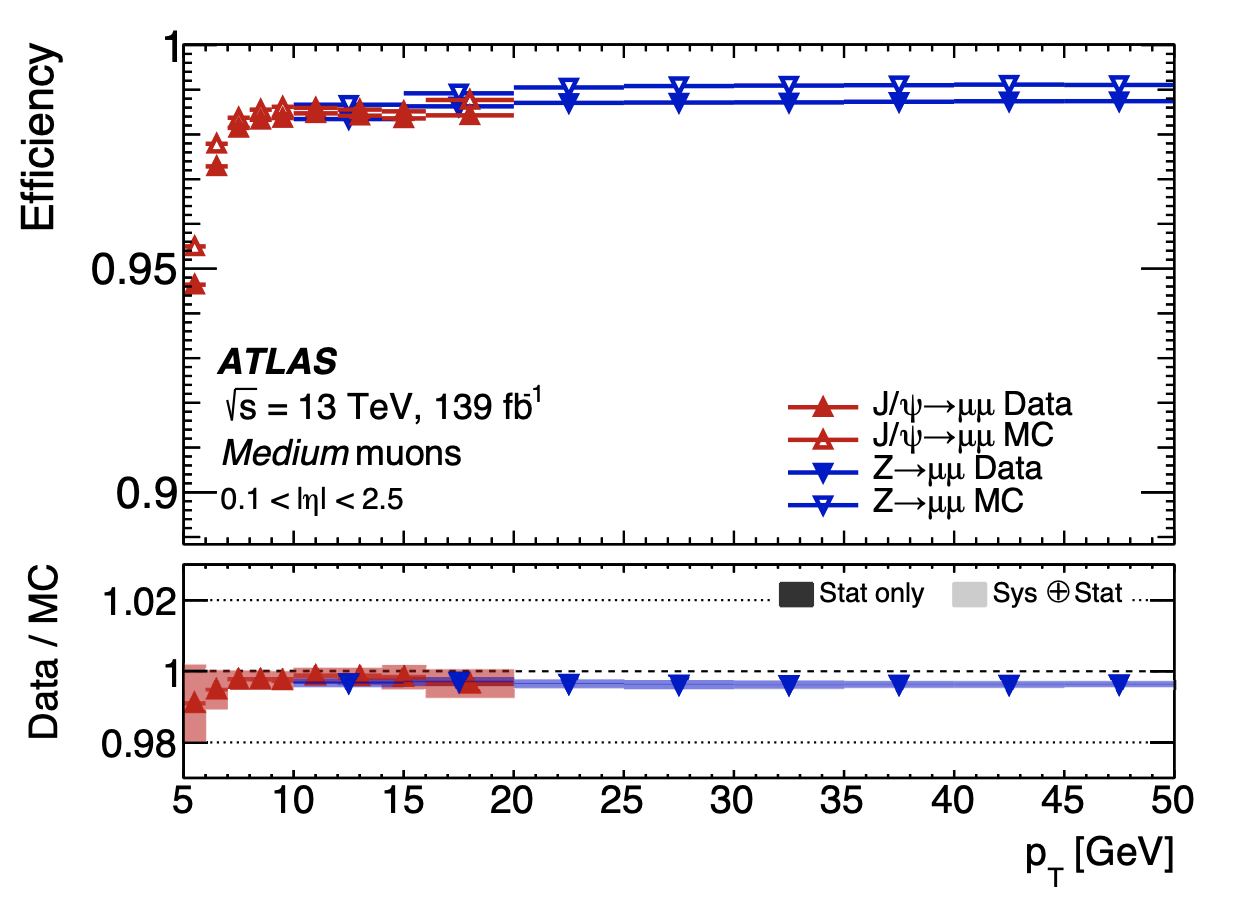
\includegraphics[width=0.9\linewidth]{fig/reco_muon_ID.png}
%\caption{\label{fig:reco:muon_ID}}
%\end{figure}

\subsubsection*{Muon isolation}
Muons from heavy particle decays are often produced in an isolated manner compared to muons from semileptonic decays, and is therefore an important tool for background rejection in many physics analyses. Muon isolation strategies are similar to that of electron in section \ref{sec:eiso}, with track-based and calorimeter-based isolation variables. Seven isolation \acs{OP}s are defined using either or both types of isolation variables \citep{reco:muon_ID}.

\section{Missing transverse momentum}
\label{sec:met}
Collisions at the \acs{LHC} happen along the $z$-axis of the ATLAS coordination system between two particle beam of equal center-of-mass energy. By conservation of momentum, the sum of transverse momenta of outgoing particles should be zero. A discrepancy between measured momentum and zero would then suggest the presence of undetectable particles, which would consist of either \acs{SM} neutrinos or some unknown \acs{BSM} particles, making missing transverse momentum (\acs{ETmiss}) an important observable to reconstruct.\\
Reconstructing \acs{ETmiss} utilizes information from fully reconstructed leptons, photons, jets and other matched track-vertex objects not associated with a prompt object (soft signals), defined with respect to the $x (y)$-axis as 
\begin{equation}
E^\mathrm{miss}_{x (y)} = -\mathlarger{\sum}_{i \in \{\text{hard objects}\}} p_{x (y),i} -\mathlarger{\sum}_{j \in \{\text{soft signals}\}} p_{x (y),j},
\end{equation}
where $p_{x(y)}$ is the $x(y)$-component of \pT for each particle \citep{reco:met}. The following observables can then be defined:
\begin{equation}
\begin{aligned}
& \mathbf{E}_\mathrm{T}^\mathrm{miss}=(E^\mathrm{miss}_{x},E^\mathrm{miss}_{y}),\\
& E_\mathrm{T}^\mathrm{miss}=|\mathbf{E}_\mathrm{T}^\mathrm{miss}|=\sqrt{(E^\mathrm{miss}_{x})^2+(E^\mathrm{miss}_{y})^2},\\
& \phi^\mathrm{miss}=\tan^{-1}(E^\mathrm{miss}_{y}/E^\mathrm{miss}_{x}),
\end{aligned}
\end{equation}
where \acs{ETmiss} represents the magnitude of the missing transverse energy vector $\mathbf{E}_\mathrm{T}^\mathrm{miss}$, and $\phi^\mathrm{miss}$ its direction in the transverse plane. The vectorial sum $\mathbf{E}_\mathrm{T}^\mathrm{miss}$ can be broken down into
\begin{equation}
\mathbf{E}_\mathrm{T}^\mathrm{miss} =
{\underbrace{
-\sum_{\substack{\text{selected}\\ \text{electrons}}} \mathbf{p}_\mathrm{T}^e
-\sum_{\substack{\text{selected}\\ \text{muons}}} \mathbf{p}_\mathrm{T}^\mu
-\sum_{\substack{\text{accepted}\\ \text{photons}}} \mathbf{p}_\mathrm{T}^\gamma
-\sum_{\substack{\text{accepted}\\ \text{\ensuremath{\tau}-leptons}}} \mathbf{p}_\mathrm{T}^\tau
-\sum_{\substack{\text{accepted}\\ \text{jets}}} \mathbf{p}_\mathrm{T}^\mathrm{jet}
}_\text{hard term}}
{\underbrace{
-\sum_{\substack{\vphantom{p}\text{unused}\\ \vphantom{p}\text{tracks}}} \mathbf{p}_\mathrm{T}^\mathrm{track}.
}_\text{soft term}}
\end{equation}
Two \acs{OP}s are defined for \acs{ETmiss}, \textit{Loose} and \textit{Tight}, with selections on jet \pT and JVT criteria \citep{reco:met2}. The \textit{Tight} \acs{OP} is used in this analysis; \textit{Tight} reduces pile-up dependence of \acs{ETmiss} by removing the phase space region containing more pile-up than hard-scatter jets, at the expense of resolution and scale at low pile-up,

\section{Overlap removal}
%\citep{reco:overlap}
Since different objects are reconstructed independently, it is possible for the same detector signals to be used to reconstruct multiple objects. An overlap removal strategy is implemented to resolve ambiguities; the overlap removal process for this analysis applies selections in \autoref{reco:overlap} sequentially, from top to bottom.

\begin{table}[!ht]
\centering
\caption{\label{reco:overlap}Overlap removal process for this analysis, applied sequentially from top to bottom.}%
\begin{tabular}{lll}
\toprule
Remove		& Keep		& Matching criteria \\
\midrule
Electron	& Electron 	& Shared ID track, $p^e_\mathrm{T,1}<p^e_\mathrm{T,2}$ \\
Muon		& Electron	& Shared ID track, CT muon \\
Electron	& Muon		& Shared ID track \\
%Photon		& Electron	& $\Delta R <0.4$ \\
%Photon		& Muon		& $\Delta R <0.4$ \\
Jet			& Electron	& $\Delta R <0.2$ \\
Electron	& Jet		& $\Delta R <0.4$ \\
Jet			& Muon		& ($\Delta R <0.2$ or ghost-associated) \& $N_\text{track}<3$ \\
Muon		& Jet		& $\Delta R < \min(0.4, 0.04+10 \text{GeV/\ensuremath{p_\mathrm{T}^\mu}})$ \\
%Jet			& Photon	& $\Delta R <0.4$ \\
\bottomrule
\end{tabular}
\end{table}



\end{document}
